\documentclass[11pt,a4paper, uplatex]{jsarticle}
%
\usepackage{amsmath,amssymb}
\usepackage{bm}
\usepackage[dvipdfmx]{graphicx}
\usepackage{ascmac}
\usepackage{listings,jlisting}
\usepackage{underscore}
\usepackage{subfig}
\lstset{
    frame=single,
    numbers=left,
    tabsize=2
}
%
\setlength{\textwidth}{\fullwidth}
\setlength{\textheight}{40\baselineskip}
\addtolength{\textheight}{\topskip}
\setlength{\voffset}{-0.2in}
\setlength{\topmargin}{0pt}
\setlength{\headheight}{0pt}
\setlength{\headsep}{0pt}
%
\newcommand{\divergence}{\mathrm{div}\,}  %ダイバージェンス
\newcommand{\grad}{\mathrm{grad}\,}  %グラディエント
\newcommand{\rot}{\mathrm{rot}\,}  %ローテーション
%
\title{メディア情報学実験・音声認識 第三週課題レポート}
\author{1510151  栁 裕太}
\date{\today}
\begin{document}

\maketitle
\section{認識対象の単語}
\begin{table}[htbp]
  \begin{center}
    \caption{実験で使用した数字単語}
    \label{tb:numbers}
    \begin{tabular}{c|c|c|c}
      \hline
      単語表記 & 単語名 & 発音 & 音素数 \\ \hline \hline
      3 & saN & /saN/ & 3 \\
      4 & yoN & /yoN/ & 3 \\
      5 & go & /go/ & 2 \\
      7 & nana & /nana/ & 4 \\
      \hline
    \end{tabular}
  \end{center}
\end{table}

\section{HMMの学習曲線}

\begin{figure}[h]
  \begin{center}
    \includegraphics[width=13.0cm]{learningCurve.ps}
    \caption{実行結果グラフ(go)}
    \label{fig:ps}
  \end{center}
\end{figure}

\section{単語認識性能評価}
\subsection{自分の声}
\begin{lstlisting}[language=c, caption=\texttt{countCorr}実行結果]
\% countCorr
(中略)
rei, 0
ichi, 0
ni, 0
saN, 10
yoN, 10
go, 10
roku, 0
nana, 10
hachi, 0
kyuu, 0
\end{lstlisting}

\subsection{他人の声}
\begin{lstlisting}[language=c, caption=\texttt{countXCorr}実行結果]
\% countXCorr m0
Evaluation start.  Wait a moment.
rei, 0
ichi, 0
ni, 0
saN, 33
yoN, 1
go, 9
roku, 0
nana, 44
hachi, 0
kyuu, 0

\% countXCorr m1
Evaluation start.  Wait a moment.
rei, 0
ichi, 0
ni, 0
saN, 22
yoN, 1
go, 32
roku, 0
nana, 30
hachi, 0
kyuu, 0

\% countXCorr m2
Evaluation start.  Wait a moment.
rei, 0
ichi, 0
ni, 0
saN, 0
yoN, 0
go, 0
roku, 0
nana, 45
hachi, 0
kyuu, 0

\% countXCorr f1
Evaluation start.  Wait a moment.
rei, 0
ichi, 0
ni, 0
saN, 4
yoN, 0
go, 15
roku, 0
nana, 47
hachi, 0
kyuu, 0

\end{lstlisting}

\section{オンライン単語認識}
\subsection{自分の声}
3, 4, 5, 7をそれぞれ3回ずつ発声し、結果を得た。
\begin{lstlisting}[language=c, caption=\texttt{recog}実行結果]
\% #saN (spoken by myself)
\% recog -20 lib/HMMList
Returnキーを押してください
Isolated Word Recogition On-The-Fly
vad_file= vadwav/10221.wav
--------------------
rank word (kana)= log-likelyhood
--------------------
 1. 3 (saN)= -1790.410712
 2. 7 (nana)= -1838.183389
 3. 4 (yoN)= -1981.794753
 4. 5 (go)= -2125.044269

ハングアップ   
Returnキーを押してください
Isolated Word Recogition On-The-Fly
vad_file= vadwav/10454.wav
--------------------
rank word (kana)= log-likelyhood
--------------------
 1. 7 (nana)= -1015.582787
 2. 3 (saN)= -1056.889629
 3. 4 (yoN)= -1113.365923
 4. 5 (go)= -1180.399190

ハングアップ   
Returnキーを押してください
Isolated Word Recogition On-The-Fly
vad_file= vadwav/10491.wav
--------------------
rank word (kana)= log-likelyhood
--------------------
 1. 3 (saN)= -2313.627728
 2. 7 (nana)= -2391.826858
 3. 4 (yoN)= -2526.148038
 4. 5 (go)= -2698.040703

ハングアップ   

\% #yoN (spoken by myself)
\% recog -20 lib/HMMList
Returnキーを押してください
Isolated Word Recogition On-The-Fly
vad_file= vadwav/10277.wav
--------------------
rank word (kana)= log-likelyhood
--------------------
 1. 4 (yoN)= -1787.122659
 2. 7 (nana)= -1816.205699
 3. 3 (saN)= -1825.196272
 4. 5 (go)= -1979.401992

ハングアップ   
Returnキーを押してください
Isolated Word Recogition On-The-Fly
vad_file= vadwav/11351.wav
--------------------
rank word (kana)= log-likelyhood
--------------------
 1. 7 (nana)= -1732.293919
 2. 4 (yoN)= -1749.738537
 3. 3 (saN)= -1758.778353
 4. 5 (go)= -1842.883630

ハングアップ   
Returnキーを押してください
Isolated Word Recogition On-The-Fly
vad_file= vadwav/11384.wav
--------------------
rank word (kana)= log-likelyhood
--------------------
 1. 4 (yoN)= -1623.474475
 2. 3 (saN)= -1675.216760
 3. 7 (nana)= -1679.459238
 4. 5 (go)= -1708.053267

ハングアップ  
\% #go (spoken by myself)
\% recog -20 lib/HMMList
Returnキーを押してください
Isolated Word Recogition On-The-Fly
vad_file= vadwav/10115.wav
--------------------
rank word (kana)= log-likelyhood
--------------------
 1. 5 (go)= -1445.805241
 2. 7 (nana)= -1490.668070
 3. 3 (saN)= -1556.722549
 4. 4 (yoN)= -1663.274652

ハングアップ   
Returnキーを押してください
Isolated Word Recogition On-The-Fly
vad_file= vadwav/12073.wav
--------------------
rank word (kana)= log-likelyhood
--------------------
 1. 5 (go)= -1349.897716
 2. 7 (nana)= -1505.549940
 3. 3 (saN)= -1550.040932
 4. 4 (yoN)= -1623.344431

ハングアップ   
Returnキーを押してください
Isolated Word Recogition On-The-Fly
vad_file= vadwav/12121.wav
--------------------
rank word (kana)= log-likelyhood
--------------------
 1. 5 (go)= -1386.920504
 2. 7 (nana)= -1426.955245
 3. 3 (saN)= -1526.620053
 4. 4 (yoN)= -1610.494881

ハングアップ   

\% #nana (spoken by myself)
\% recog -20 lib/HMMList
Returnキーを押してください
Isolated Word Recogition On-The-Fly
vad_file= vadwav/10306.wav
--------------------
rank word (kana)= log-likelyhood
--------------------
 1. 7 (nana)= -1384.627282
 2. 3 (saN)= -1536.170493
 3. 4 (yoN)= -1621.792248
 4. 5 (go)= -1777.863372

ハングアップ   
Returnキーを押してください
Isolated Word Recogition On-The-Fly
vad_file= vadwav/12208.wav
--------------------
rank word (kana)= log-likelyhood
--------------------
 1. 7 (nana)= -1565.372470
 2. 3 (saN)= -1864.963177
 3. 4 (yoN)= -1942.985780
 4. 5 (go)= -2001.167651

ハングアップ   
Returnキーを押してください
Isolated Word Recogition On-The-Fly
vad_file= vadwav/12236.wav
--------------------
rank word (kana)= log-likelyhood
--------------------
 1. 7 (nana)= -1732.933940
 2. 3 (saN)= -1986.133111
 3. 4 (yoN)= -2071.052025
 4. 5 (go)= -2194.124920

ハングアップ   
\end{lstlisting}

\subsection{他人の声}
今回の実験では、友人の張氏と浅津氏の2人に協力して頂き、3, 4, 5, 7の順に発声してもらった。
\subsubsection{張氏の場合}
\begin{lstlisting}[language=c, caption=\texttt{recog}実行結果(張氏)]
Returnキーを押してください
Isolated Word Recogition On-The-Fly
vad_file= vadwav/39826.wav
--------------------
rank word (kana)= log-likelyhood
--------------------
 1. 3 (saN)= -1505.069939
 2. 7 (nana)= -1586.825035
 3. 5 (go)= -1748.309120
 4. 4 (yoN)= -1753.374475

ハングアップ   
Returnキーを押してください
Isolated Word Recogition On-The-Fly
vad_file= vadwav/39885.wav
--------------------
rank word (kana)= log-likelyhood
--------------------
 1. 5 (go)= -1344.840856
 2. 4 (yoN)= -1361.261114
 3. 7 (nana)= -1455.075794
 4. 3 (saN)= -1500.914987

ハングアップ   
Returnキーを押してください
Isolated Word Recogition On-The-Fly
vad_file= vadwav/39936.wav
--------------------
rank word (kana)= log-likelyhood
--------------------
 1. 7 (nana)= -1161.868159
 2. 4 (yoN)= -1187.774808
 3. 3 (saN)= -1208.448915
 4. 5 (go)= -1232.254232

ハングアップ   
Returnキーを押してください
Isolated Word Recogition On-The-Fly
vad_file= vadwav/39971.wav
--------------------
rank word (kana)= log-likelyhood
--------------------
 1. 7 (nana)= -877.720638
 2. 4 (yoN)= -938.691815
 3. 3 (saN)= -943.252832
 4. 5 (go)= -970.624385

ハングアップ   
\end{lstlisting}

\subsubsection{浅津氏の場合}
\begin{lstlisting}[language=c, caption=\texttt{recog}実行結果(浅津氏)]
#3, 4, 5, 7の順に発声
Returnキーを押してください
Isolated Word Recogition On-The-Fly
vad_file= vadwav/44822.wav
--------------------
rank word (kana)= log-likelyhood
--------------------
 1. 7 (nana)= -1955.394600
 2. 3 (saN)= -1960.798787
 3. 4 (yoN)= -2085.992983
 4. 5 (go)= -2102.686864

ハングアップ   
Returnキーを押してください
Isolated Word Recogition On-The-Fly
vad_file= vadwav/44962.wav
--------------------
rank word (kana)= log-likelyhood
--------------------
 1. 7 (nana)= -951.017733
 2. 3 (saN)= -979.229846
 3. 4 (yoN)= -1051.388855
 4. 5 (go)= -1086.196301

ハングアップ   
Returnキーを押してください
Isolated Word Recogition On-The-Fly
vad_file= vadwav/45027.wav
--------------------
rank word (kana)= log-likelyhood
--------------------
 1. 7 (nana)= -951.803934
 2. 3 (saN)= -983.027531
 3. 4 (yoN)= -994.104035
 4. 5 (go)= -1012.153328

ハングアップ   
Returnキーを押してください
Isolated Word Recogition On-The-Fly
vad_file= vadwav/45062.wav
--------------------
rank word (kana)= log-likelyhood
--------------------
 1. 7 (nana)= -878.557397
 2. 3 (saN)= -1032.259370
 3. 5 (go)= -1033.311989
 4. 4 (yoN)= -1044.670763

ハングアップ   
\end{lstlisting}

\subsection{考察}
今回のオンライン音声認識では、自分の発声ではほぼ安定した結果を得ることができた。
しかしながら、友人に発声してもらったところ、判定がかなり不安定な結果となった。

張氏では、中国人留学生で発音が独特だった影響か、特に5の発声では5の最尤順位が最下位となった。
また浅津氏の場合では、すべての発声において7が最尤と判定され、
更にこちらでも5の発声時に5が最尤順位が最下位となった。
これより5においては、
自分の発話性が独特であった影響によって判定が不安定になっている可能性が考えられた。

また浅津氏の場合では、3, 4, 5の発話において、最尤順位がすべて7, 3, 4, 5の順序になっていた。
これは、浅津氏の発話性による影響を受けたものと考えている。

日本人である浅津氏と中国人留学生である張氏の2者に手伝って頂いたが、
最尤順位が正しい数字となる回数では張氏の方が多かった。
これは、音声認識の観点では中国語訛りの日本語であろうと、
ある程度発話性によっては対応できる可能性を示唆しているのではないかと考えている。
同様に日本人の発話においても、
発話性によっては判定が不安定になることも同時に示唆していると解釈した。

\section{実験のポイント}
音声認識において、音声入力から判定までの流れを学ぶことと、過程にて活用する数理モデルの実践

\section{よくわかったこと}
基本的な処理としては、パターンマッチングによってもっとも近い単語を調べているということ

\section{よくわからなかったこと}
単語のみならず、文脈を活用した単語の推測・判定

\section{要望}
システムの信頼性をもう少し改善してほしかった。
不具合によって録音不可能になって実験作業に手間取るケースがしばしばあった。

\section{感想・その他}
特になし

\end{document}
